%%%%%%%%%%%%%%%%%%%%%%%%%%%%%%%%%%%%%%%%%
% Journal Article
% LaTeX Template
% Version 1.3 (9/9/13)
%
% This template has been downloaded from:
% http://www.LaTeXTemplates.com
%
% Original author:
% Frits Wenneker (http://www.howtotex.com)
%
% License:
% CC BY-NC-SA 3.0 (http://creativecommons.org/licenses/by-nc-sa/3.0/)
%
%%%%%%%%%%%%%%%%%%%%%%%%%%%%%%%%%%%%%%%%%

%----------------------------------------------------------------------------------------
%	PACKAGES AND OTHER DOCUMENT CONFIGURATIONS
%----------------------------------------------------------------------------------------

\documentclass[twoside]{article}

\usepackage{biblatex}
\bibliography{project.bib}

\usepackage[sc]{mathpazo} % Use the Palatino font
\usepackage[T1]{fontenc} % Use 8-bit encoding that has 256 glyphs
\usepackage[utf8]{inputenc}
\linespread{1.05} % Line spacing - Palatino needs more space between lines
\usepackage{microtype} % Slightly tweak font spacing for aesthetics

\usepackage[hmarginratio=1:1,top=32mm,columnsep=20pt]{geometry} % Document margins
\usepackage{multicol} % Used for the two-column layout of the document
\usepackage[hang, small,labelfont=bf,up,textfont=it,up]{caption} % Custom captions under/above floats in tables or figures
\usepackage{booktabs} % Horizontal rules in tables
\usepackage{float} % Required for tables and figures in the multi-column environment - they need to be placed in specific locations with the [H] (e.g. \begin{table}[H])
\usepackage{hyperref} % For hyperlinks in the PDF

\usepackage{lettrine} % The lettrine is the first enlarged letter at the beginning of the text
\usepackage{paralist} % Used for the compactitem environment which makes bullet points with less space between them

\usepackage{listings}
   \usepackage[pdftex]{graphicx} 

\usepackage{abstract} % Allows abstract customization
\renewcommand{\abstractnamefont}{\normalfont\bfseries} % Set the "Abstract" text to bold
\renewcommand{\abstracttextfont}{\normalfont\small\itshape} % Set the abstract itself to small italic text

\usepackage{titlesec} % Allows customization of titles
\renewcommand\thesection{\Roman{section}} % Roman numerals for the sections
\renewcommand\thesubsection{\Roman{subsection}} % Roman numerals for subsections
\titleformat{\section}[block]{\large\scshape\centering}{\thesection.}{1em}{} % Change the look of the section titles
\titleformat{\subsection}[block]{\large}{\thesubsection.}{1em}{} % Change the look of the section titles

\usepackage{fancyhdr} % Headers and footers
\pagestyle{fancy} % All pages have headers and footers
\fancyhead{} % Blank out the default header
\fancyfoot{} % Blank out the default footer
\fancyhead[C]{LINGI2141 - Individual Project $\bullet$ December 2013 } % Custom header text
\fancyfoot[RO,LE]{\thepage} % Custom footer text

%----------------------------------------------------------------------------------------
%	TITLE SECTION
%----------------------------------------------------------------------------------------

\title{\vspace{-15mm}\fontsize{24pt}{10pt}\selectfont\textbf{LINGI2141 - Individual Project \\Analysis of APT-GET}} % Article title

\author{
\large
\textsc{Benoît Baufays}\\[2mm] % Your name
\normalsize Université Catholique de Louvain \\ % Your institution
\vspace{-5mm}
}
\date{}

%----------------------------------------------------------------------------------------

\begin{document}

\maketitle % Insert title

\thispagestyle{fancy} % All pages have headers and footers

%----------------------------------------------------------------------------------------
%	ABSTRACT
%----------------------------------------------------------------------------------------

\begin{abstract}

This paper will deal with analysing the managing software apt-get wich are deployed on several linux distributions 

\end{abstract}

%----------------------------------------------------------------------------------------
%	ARTICLE CONTENTS
%----------------------------------------------------------------------------------------

\begin{multicols}{2} % Two-column layout throughout the main article text

\section{Introduction}

\lettrine[nindent=0em,lines=3]{A} pt-get is a software develloped for linux OS to centralize the management of your software.  Apt-get install packages  containing precompiled code, configuration files, and meta-information about the package.  Because it is not very usefull to manage manually all your packages, apt-get was created.  With him, you can update your system and yours packages but you can also install or remove packages.  The utility of apt-get is the management of the dependencies and, with one program, you can maintain your system up to date.

\section{Apt-get}
Apt-get have several commands, depending on what you want to do.
\begin{itemize}
	\item update : with this command, apt-get search, on remotes servers, the last version for all packets.  It get also the entire list of packets you can install via apt-get;
	\item upgrade or dist-upgrade : with this command, apt-get downloads packets installed on your system wich are to be updated.  The difference between the command "upgrade" and "dist-upgrade" is that, whit hthe first, apt-get doesn't install new packages.  For example, some packages must requires new dependencies.  If you update with the first command, apt-get doesn't install new dependencies and, of course, doesn't update the packet.  In other hand, with the second command, apt-get install all dependencies and update all packages;
	\item install : with this command, you can install new package.  Apt-get search for dependencies and install the package and the required packages;
	\item remove : with this command, apt-get remove the package mentionned.  It can also remove packages wich are not still required on your system.  For example, if a package is only installed because it is a dependency for an other package and you remove this package, it is not require to have the dependency's package on your system.
\end{itemize}
Apt-get have several others command but the main has be presented below.  To analyse how apt-get works and deal with network, we will use the same order presented in the list below.  But, before, we discuss about the IPv 6 and apt-get.

\section{Apt-get and IPv6}
To know where it must searching informations about packages, apt-get have one file "/etc/apt/sources.list" which contains addresses of servers.  According to several bloggers, apt-get have some troubles with IPv6 because some servers have no Ipv6 address or the ISP doesn't support it.\\
To verify this information, we have used dig to send a DNS request to archive.ubuntu.com, the main server for every sources.\\ \\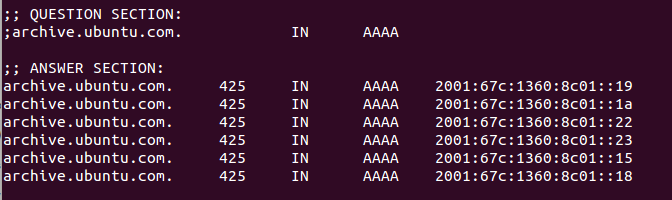
\includegraphics[scale=0.3]{pictures/DNS_info.png}



As we can see, archive.ubuntu.com have several IPv6 address, the problem do not come form that.  When we go deeper in the code of apt-get, we see that some functionnalities are still using IPv4 libraries.

\section{Apt-get analysis}
\subsection{Update}
\subsubsection{DNS Request}
With this command, apt-get read first the file containing all server's name.  With this information, it sends DNS request to know IP address of each server. \\ \\ 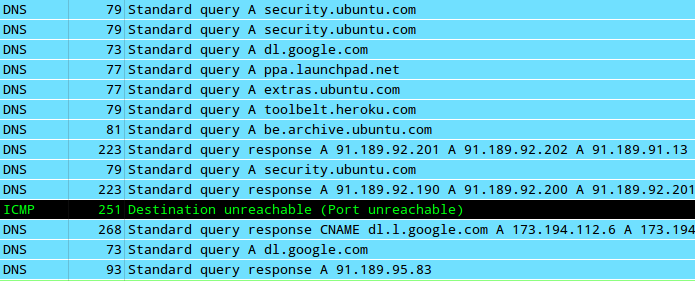
\includegraphics[scale=0.32]{pictures/dns_update.png}

As we can see, Apt-get send first all his DNS requests before contacting servers.  We see also that dl.google.com, an entry that we have added manually to access to packages from Google (GoogleTalk, ...) is, in reality, reachable via dl.l.google.com.  Finally, we can see that apt-get send twice the DNS request about dl.google.com.  It's not beacause it doesn't receive the response but because we have added twice this entry in the config file.\\
To test the DNS system, we have put manually a arbitrary IP address for the second DNS server.  This test is visible in the schema below with the "Destination unreachable" message.  After that, apt-get doesn't reuse this IP adress to send DNS query.\\
When we analysing packets receive by apt-get, we see that the time life of the information is 3 minutes 30.  Also, we see that it receive more than one IP address for every server name.  With this solution, apt-get doesn't want  to resend a DNS query if a IP adress down.  With multiple IP adresses, it can also  use multi threading and request informations on multiple servers.\\
\subsubsection{Getting information}
With the IP address, apt-get can now getting informations about packages.  These informations are getting in two step.\\ \\ 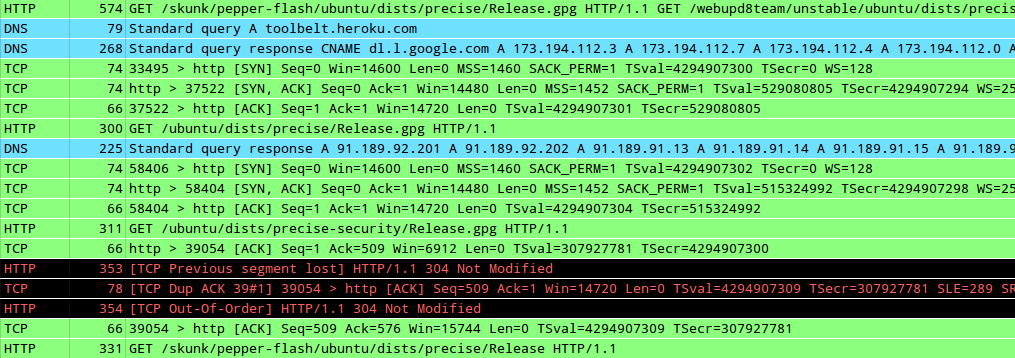
\includegraphics[scale=0.2]{pictures/update_get_1.png}
First, as we can see in the schema above, apt-get get some files with HTTP 1.1.  Before, it do a three handsake (SYN, SYN-ACK,ACK) to open the connection.  For example, after having open a connection with the server, apt-get download "http://extras.ubuntu.com/ubuntu/dists/precise/Release".  Because it's a file readable, we have downloaded it to see how apt-get works.\\ \\ 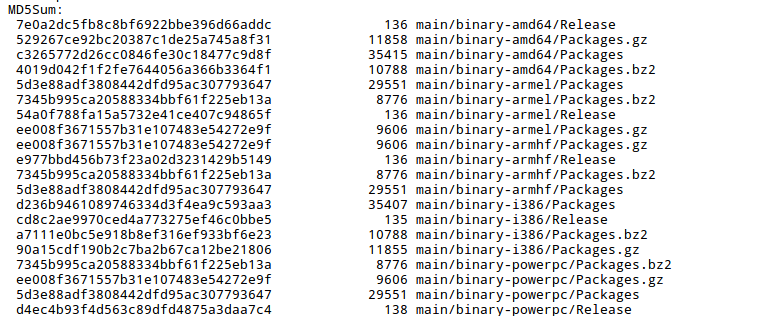
\includegraphics[scale=0.3]{pictures/update_first_file.png}
For each subfiles, containing informations about packages, it receive the MD5 sum or the SHA1 sum (not present in the schema), the size of the file you will download and, finally, the path to download the file.  In fact, it's not a file, it's a archive.  With this solution, ubuntu compress informations.\\
With the schema above, we can also see that apt-get still send and receive DNS query while we have noticed, i nthe previous subsection that apt-get send all his queries before getting informations about packages.  It's true for main addresses but, for addresses you have added manually, apt-get begin to download informations about packages before it have finished DNS queries for personnalized addresses.\\
We see also how apt-get retrieve from lost packets (dark line in the schema).  Because apt-get use TCP, it receive first a packet that indicate the lsot segment.  With this information, apt-get send back a duplication acknowledgement.  In this example, we have added a delay for some packets and we can see that, after the duplication acknowledgement, apt-get receive the lost packet and TCp say "TCP out of order ".  it means that this packet arrive not in the correct order.  it's logical because with put a delay for one packet.\\
After having downloaded the main file, apt-get download archive listed in the main file.  If you download also the archive, you can see that it contains one file, listing all packages and informations about each : checksum, name, description, last version, dependencies, ...  With this file, apt-get can updated his local informations and test if you have the last version.  If not, it's mark the package.\\
\subsection{upgrade}
Upgrade is just a succession of install command for every package which requires an update.  So, you can find our analysis of install in the next section.

\subsection{Install}
To analysis packets and network activity, we have installed a package with dependencies.\\ 
Again, apt-get work in two step : DNS query and download.  After checking that the requested package exist in its database, it extracts, from informations taken during the update command, the address of the server where it can download package.\\
In our example, it search also informations about dependencies and if not installed, it adds these packages to download.  In fact, apt-get have a cache system and if the connection is closed before it have finished to download, you can restart the command and apt-get resumes with the last packet received.  It is possible thanks to HTTP protocol that allow to resume download, if this option is enabled on the distant server.  Here, ubuntu servers have enabled this option.\\ 
\subsubsection{DNS Request}
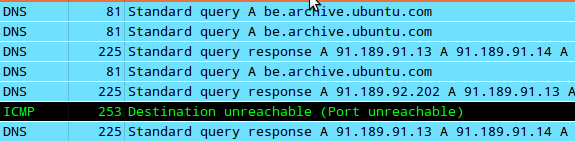
\includegraphics[scale=0.4]{pictures/install_dns.png}
Like in the subsection "update", we see that apt-get send DNS request twice.  Here, it sends to the principal and the second DNS server address.  Again, it receives an "Destination unreachable" packet for the second DNS server.\\
We can also see that it sends a third time a DNS request to "archive.ubuntu.com".  This time, it sends to the principal DNS server and it's for a dependency package.  He could have used the information from the previous query, but it's a consequence of multi thread : to increase the speed of downloading, apt-get download two packages simultaneously.\\
\subsubsection{Download packages}
After having IP adresses of servers where apt-get can download packages, apt-get open a TCP connection with the server to download packages.\\ \\ 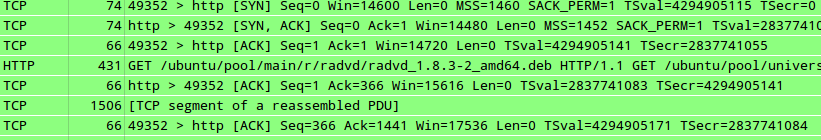
\includegraphics[scale=0.27]{pictures/install_download.png}
Like every TCP connections, it starts with the three handsake between the client and the server (SYN,SYN-ACK,ACK).  After the connection is opened, apt-get send a HTTP request to download the package.\\
As yo ucan see, the server sends a lot of packets and our system send back acknowledgment but not for every packet.  In fact, Wireshark indicates "TCP segment of a reassembled PDU".  This label notices that Wireshark reassembles a higher level protocol packets.  In this example, it's normal to see this label because the reply of the HTTP request take more than one packet.  When we analysis this reassembled packet, we can see the next sequence number and the acknowledgment number.  When we get the next packet sended by our system, we see that it's a ACK packet with the correct number linked to the previous reassembled packet.\\
At the end of the download, our system receive a HTTP packet with the type of the file downloaded.  in this exmaple, it's an application/x-debian-package, a binary package.\\
When all packages are downloaded, we see that our system close the TCP connection with FIN-ACK,FIN-ACK,ACK packets.\\  With this sequence, we see that apt-get doesn't send informations about your installation or errors.  To check more deeper this preliminary conclusion, we have analysed networck activity during the last phase of install, where apt-get install packages on our system.  We see not packets from apt-get program or from Ubuntu.  When we stop the processus, we also don't see packets.  We can see that apt-get doesn't send informations about your system\\
\subsection{Remove}
Normally, apt-get should not send or receive packets when you remove a package but we wondered if, for statistical reasons, Ubuntu track remove command.  For example, Ubuntu can track remove action to compute ranking for every package.  If you open Software Manager, an UI application for apt-get, yo ucan see a ranking for every main packages.\\
After having remove small packages, we see that, with Wireshark, no packets was echanged.  So, we remove kernel package (previous version of course) and, again, no packets was echanged.  We can say that apt-get doesn't track remove action.\\


%------------------------------------------------

%------------------------------------------------

%------------------------------------------------


%----------------------------------------------------------------------------------------
%	REFERENCE LIST
%----------------------------------------------------------------------------------------

\printbibliography

%----------------------------------------------------------------------------------------

\end{multicols}

\end{document}
